\chapter{Day 2 Motions}
\label{ch-day2}




% ******************************************************************
% ******************************************************************
% ******************************************************************
\clearpage
\newpage
\section{Deconvolution 1D Motions}
\label{Deconvolution_1D_Motions}


\subsection{Free field 1D model, deconvolution 1D motion, model with DRM}
\label{Free_fields_1D_model_with_DRM1}


The Real-ESSI input files for this example are available 
\href{https://github.com/yuan-energy/Real-ESSI-Short-Course-Examples/tree/master/short-course-examples/Day2/Deconvolution_1D_Motions/Free_fields_1D_model_with_DRM}{HERE}. 
The compressed package of Real-ESSI input files for this example is available 
\href{https://github.com/yuan-energy/Real-ESSI-Short-Course-Examples/blob/master/short-course-examples/Day2/Deconvolution_1D_Motions/Free_fields_1D_model_with_DRM/Free_fields_1D_model_with_DRM.tgz?raw=true}{HERE}. 

The Modeling parameters are listed.
\begin{itemize}
  \item Elastic Material Properties 
  \begin{itemize}
    \item Mass density, $\rho$, \enspace \enspace 2000 $kg/m^3$
    \item Young's modulus, $E$, \enspace \enspace 200 MPa
    \item Poisson's ratio, $\nu$, \enspace \enspace 0.1
  \end{itemize}
\end{itemize}


\begin{figure}[H]
  \centering
  \includegraphics[width = 0.8cm]{./Figure-files/Day2/Deconvolution_1D_Motions/Free_fields_1D_model_with_DRM/overview.png}
  \caption{Simulation Model}
  \label{fig_decon_1D_motion_1D_model1}
\end{figure}

The illustration results of the simulation is shown in Fig.~\ref{fig_decon_1D_motion_1D_model}.
As shown in the results, outside the DRM layer, there is no outgoing waves. 

\begin{figure}[H]
  \centering
  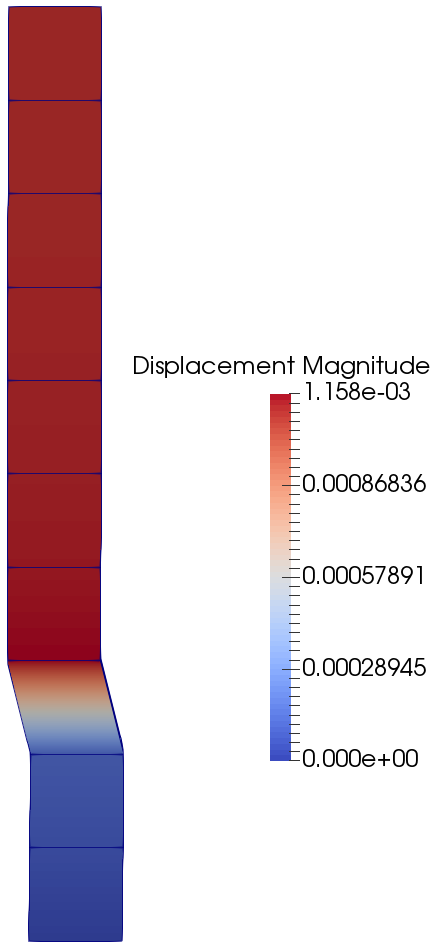
\includegraphics[width = 5cm]{./Figure-files/Day2/Deconvolution_1D_Motions/Free_fields_1D_model_with_DRM/DRM1D_results.png}
  \caption{Simulation Model}
  \label{fig_decon_1D_motion_1D_model_results}
\end{figure}


% ******************************************************************
% ******************************************************************
% ******************************************************************
\clearpage
\newpage
\subsection{Free field 3D model, deconvolution 1D motion, model with DRM}
\label{Free_fields_3D_model_with_DRM1}


The Real-ESSI input files for this example are available 
\href{https://github.com/yuan-energy/Real-ESSI-Short-Course-Examples/tree/master/short-course-examples/Day2/Deconvolution_1D_Motions/Free_fields_3D_model_with_DRM}{HERE}. 
The compressed package of Real-ESSI input files for this example is available 
\href{https://github.com/yuan-energy/Real-ESSI-Short-Course-Examples/blob/master/short-course-examples/Day2/Deconvolution_1D_Motions/Free_fields_3D_model_with_DRM/Free_fields_3D_model_with_DRM.tgz?raw=true}{HERE}. 

The Modeling parameters are listed.
\begin{itemize}
  \item Elastic Material Properties 
  \begin{itemize}
    \item Mass density, $\rho$, \enspace \enspace 2000 $kg/m^3$
    \item Young's modulus, $E$, \enspace \enspace 200 MPa
    \item Poisson's ratio, $\nu$, \enspace \enspace 0.1
  \end{itemize}
\end{itemize}


\begin{figure}[H]
  \centering
  \includegraphics[width = 8cm]{./Figure-files/Day2/Deconvolution_1D_Motions/Free_fields_3D_model_with_DRM/overview.png}
  \caption{Simulation Model}
  \label{fig_decon_1D_motion_3D_model1}
\end{figure}


The illustration results of free field DRM 3D Model under 1D motion is shown 
in Fig.~\ref{fig_day2_DRM3D_results}. 

\begin{figure}[H]
  \centering
  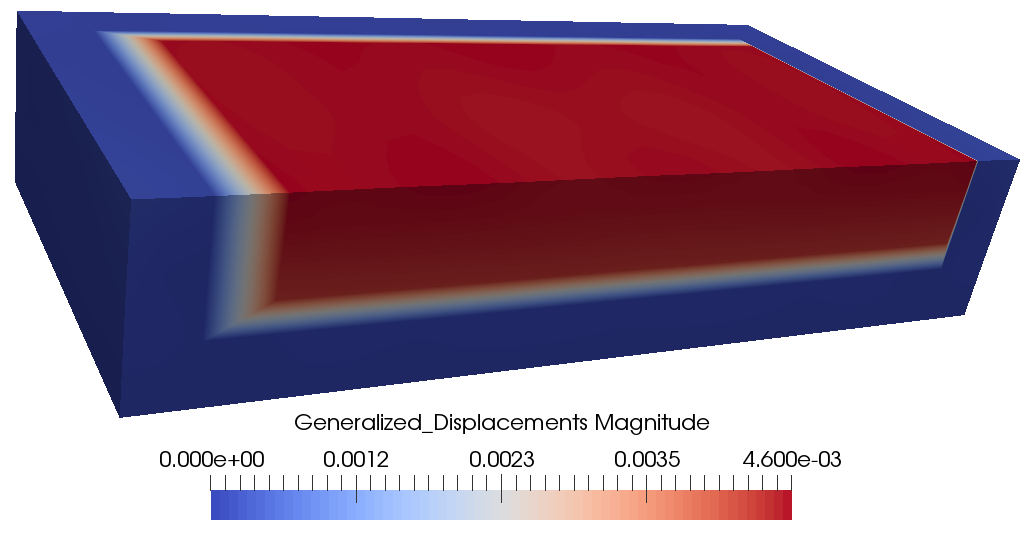
\includegraphics[width = 10cm]{./Figure-files/Day1/Preprocess_examples_with_Gmsh/example4/DRM3D_results.png}
  \caption{Simulation Model DRM 2D}
  \label{fig_day2_DRM3D_results}
\end{figure}



% ******************************************************************
% ******************************************************************
% ******************************************************************
\clearpage
\newpage
\subsection{ESSI 3D building model, deconvolution 1D model, solid model with DRM}
\label{Earthquake_Soil-Structure_Interaction_3D_Model_with_DRM1}

The Real-ESSI input files for this example are available 
\href{https://github.com/yuan-energy/Real-ESSI-Short-Course-Examples/tree/master/short-course-examples/Day2/Deconvolution_1D_Motions/Earthquake_Soil-Structure_Interaction_3D_Model_with_DRM}{HERE}. 
The compressed package of Real-ESSI input files for this example is available 
\href{https://github.com/yuan-energy/Real-ESSI-Short-Course-Examples/blob/master/short-course-examples/Day2/Deconvolution_1D_Motions/Earthquake_Soil-Structure_Interaction_3D_Model_with_DRM/Earthquake_Soil-Structure_Interaction_3D_Model_with_DRM.tgz?raw=true}{HERE}. 

The Modeling parameters are listed.
\begin{itemize}
  \item Elastic Soil Material Properties 
  \begin{itemize}
    \item Mass density, $\rho$, \enspace \enspace 2000 $kg/m^3$
    \item Young's modulus, $E$, \enspace \enspace 200 MPa
    \item Poisson's ratio, $\nu$, \enspace \enspace 0.1
  \end{itemize}
  \item Elastic Structure Material Properties 
  \begin{itemize}
    \item Mass density, $\rho$, \enspace \enspace 2500 $kg/m^3$
    \item Young's modulus, $E$, \enspace \enspace 20 GPa
    \item Poisson's ratio, $\nu$, \enspace \enspace 0.1
  \end{itemize}
\end{itemize}

\begin{figure}[H]
  \centering
  \includegraphics[width = 8cm]{./Figure-files/Day2/Deconvolution_1D_Motions/Earthquake_Soil-Structure_Interaction_3D_Model_with_DRM/overview.png}
  \caption{Simulation Model}
  \label{fig_decon_1D_motion_3D_model2}
\end{figure}


The illustration results of DRM 3D Solid Structure Model  under 1D motion is shown 
in Fig.~\ref{fig_decon_1D_motion_3D_model_solid_structure}. 

\begin{figure}[H]
  \centering
  \includegraphics[width = 10cm]{./Figure-files/Day2/Deconvolution_1D_Motions/Earthquake_Soil-Structure_Interaction_3D_Model_with_DRM/DRM3D_results_1Dmotion.png}
  \caption{Simulation Model}
  \label{fig_decon_1D_motion_3D_model_solid_structure}
\end{figure}






% ******************************************************************
% ******************************************************************
% ******************************************************************
\clearpage
\newpage
\subsection{ESSI 3D building model, deconvolution 1D model, shell model with DRM}
\label{Earthquake_Soil-Structure_Interaction_3D_Model_with_DRM2}

The Real-ESSI input files for this example are available 
\href{https://github.com/yuan-energy/Real-ESSI-Short-Course-Examples/tree/master/short-course-examples/Day2/Deconvolution_1D_Motions/Shell_Structure_Soil_Interaction_3D_DRM}{HERE}. 
The compressed package of Real-ESSI input files for this example is available 
\href{https://github.com/yuan-energy/Real-ESSI-Short-Course-Examples/blob/master/short-course-examples/Day2/Deconvolution_1D_Motions/Shell_Structure_Soil_Interaction_3D_DRM/Shell_Structure_Soil_Interaction_3D_DRM.tgz?raw=true}{HERE}. 

The Modeling parameters are listed.
\begin{itemize}
  \item Elastic Soil Material Properties 
  \begin{itemize}
    \item Mass density, $\rho$, \enspace \enspace 2000 $kg/m^3$
    \item Young's modulus, $E$, \enspace \enspace 200 MPa
    \item Poisson's ratio, $\nu$, \enspace \enspace 0.1
  \end{itemize}
  \item Elastic Structure Material Properties 
  \begin{itemize}
    \item Mass density, $\rho$, \enspace \enspace 2500 $kg/m^3$
    \item Young's modulus, $E$, \enspace \enspace 20 GPa
    \item Poisson's ratio, $\nu$, \enspace \enspace 0.1
  \end{itemize}
\end{itemize}

\begin{figure}[H]
  \centering
  \includegraphics[width = 8cm]{./Figure-files/Day2/Deconvolution_1D_Motions/Shell_Structure_Soil_Interaction_3D_DRM/overview.png}
  \caption{Simulation Model}
  \label{fig_decon_1D_motion_3D_model_shell1}
\end{figure}


The illustration results of DRM 3D shell Structure Model under 1D motion is shown 
in Fig.~\ref{fig_decon_1D_motion_3D_model_solid_shell_structure}. 

\begin{figure}[H]
  \centering
  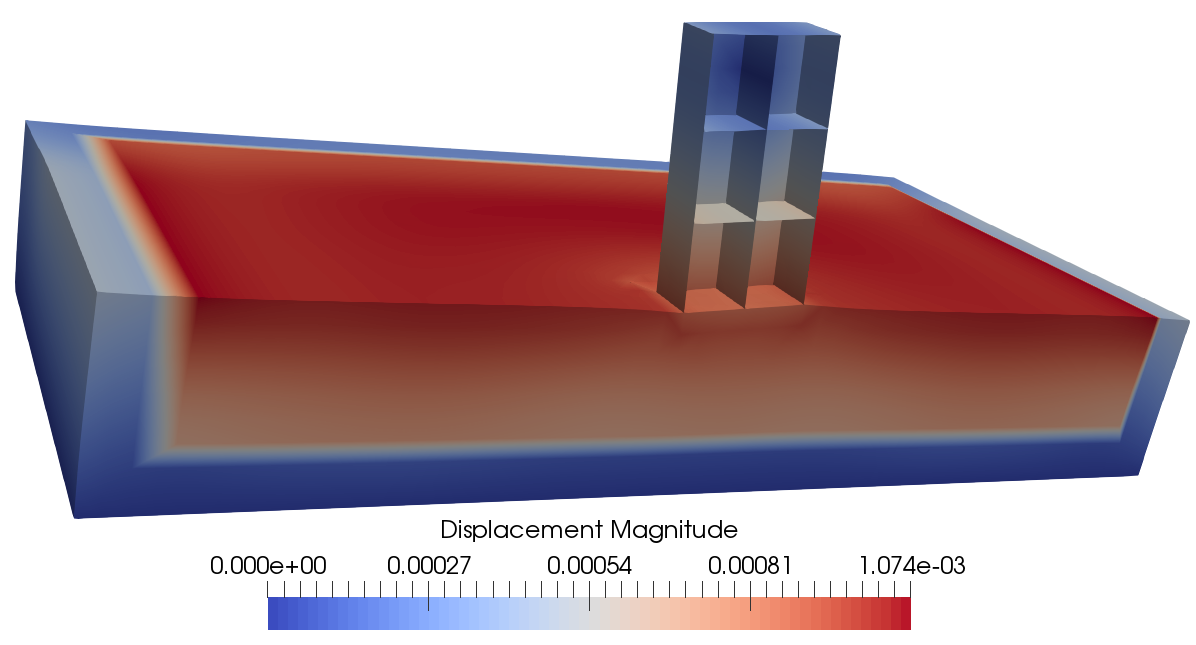
\includegraphics[width = 10cm]{./Figure-files/Day2/Deconvolution_1D_Motions/Shell_Structure_Soil_Interaction_3D_DRM/shell_DRM3D.png}
  \caption{Simulation Model}
  \label{fig_decon_1D_motion_3D_model_solid_shell_structure}
\end{figure}



























% ******************************************************************
% ******************************************************************
% ******************************************************************
\clearpage
\newpage
\section{Deconvolution 3$\times$1D Motions}
\label{Deconvolution_3by1D_Motions}
\subsection{Free field 1D model, deconvolution  3$\times$1D motion, model with DRM}
\label{Free_fields_1D_model_with_DRM2}

The Real-ESSI input files for this example are available 
\href{https://github.com/yuan-energy/Real-ESSI-Short-Course-Examples/tree/master/short-course-examples/Day2/Deconvolution_3by1D_Motions/Free_fields_1D_model_with_DRM}{HERE}. 
The compressed package of Real-ESSI input files for this example is available 
\href{https://github.com/yuan-energy/Real-ESSI-Short-Course-Examples/blob/master/short-course-examples/Day2/Deconvolution_3by1D_Motions/Free_fields_1D_model_with_DRM/Free_fields_1D_model_with_DRM.tgz?raw=true}{HERE}. 

The Modeling parameters are listed.
\begin{itemize}
  \item Elastic Material Properties 
  \begin{itemize}
    \item Mass density, $\rho$, \enspace \enspace 2000 $kg/m^3$
    \item Young's modulus, $E$, \enspace \enspace 200 MPa
    \item Poisson's ratio, $\nu$, \enspace \enspace 0.1
  \end{itemize}
\end{itemize}

\begin{figure}[H]
  \centering
  \includegraphics[width = 0.8cm]{./Figure-files/Day2/Deconvolution_3by1D_Motions/Free_fields_1D_model_with_DRM/overview.png}
  \caption{Simulation Model}
  \label{fig_decon_1D_motion_1D_model2}
\end{figure}

The illustration results of the simulation is shown in Fig.~\ref{fig_decon_1D_motion_1D_model}.
As shown in the results, outside the DRM layer, there is no outgoing waves. 

\begin{figure}[H]
  \centering
  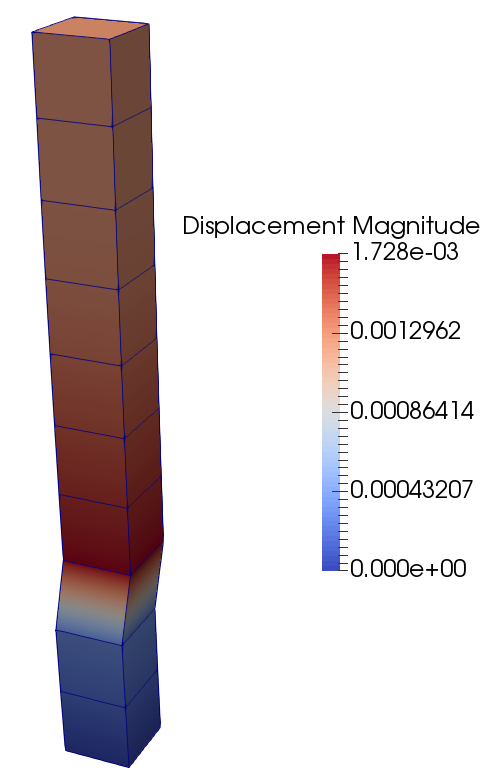
\includegraphics[width = 7cm]{./Figure-files/Day2/Deconvolution_3by1D_Motions/Free_fields_1D_model_with_DRM/DRM1D_Motion3D.png}
  \caption{Simulation Model}
  \label{fig_decon_3D_motion_1D_model_results}
\end{figure}


% ******************************************************************
% ******************************************************************
% ******************************************************************
\clearpage
\newpage
\subsection{Free field 3D model, deconvolution  3$\times$1D motion, model with DRM}
\label{Free_fields_3D_model_with_DRM2}

The Real-ESSI input files for this example are available 
\href{https://github.com/yuan-energy/Real-ESSI-Short-Course-Examples/tree/master/short-course-examples/Day2/Deconvolution_3by1D_Motions/Free_fields_3D_model_with_DRM}{HERE}. 
The compressed package of Real-ESSI input files for this example is available 
\href{https://github.com/yuan-energy/Real-ESSI-Short-Course-Examples/blob/master/short-course-examples/Day2/Deconvolution_3by1D_Motions/Free_fields_3D_model_with_DRM/Free_fields_3D_model_with_DRM.tgz?raw=true}{HERE}. 

The Modeling parameters are listed.
\begin{itemize}
  \item Elastic Soil Material Properties 
  \begin{itemize}
    \item Mass density, $\rho$, \enspace \enspace 2000 $kg/m^3$
    \item Young's modulus, $E$, \enspace \enspace 200 MPa
    \item Poisson's ratio, $\nu$, \enspace \enspace 0.1
  \end{itemize}
\end{itemize}


\begin{figure}[H]
  \centering
  \includegraphics[width = 8cm]{./Figure-files/Day2/Deconvolution_3by1D_Motions/Free_fields_3D_model_with_DRM/overview.png}
  \caption{Simulation Model}
  \label{fig_decon_3by1D_motion_3D_model}
\end{figure}

The illustration results of the simulation is shown in Fig.~\ref{fig_decon_3D_motion_3D_model_results_free_field}.
As shown in the results, outside the DRM layer, there is no outgoing waves. 

\begin{figure}[H]
  \centering
  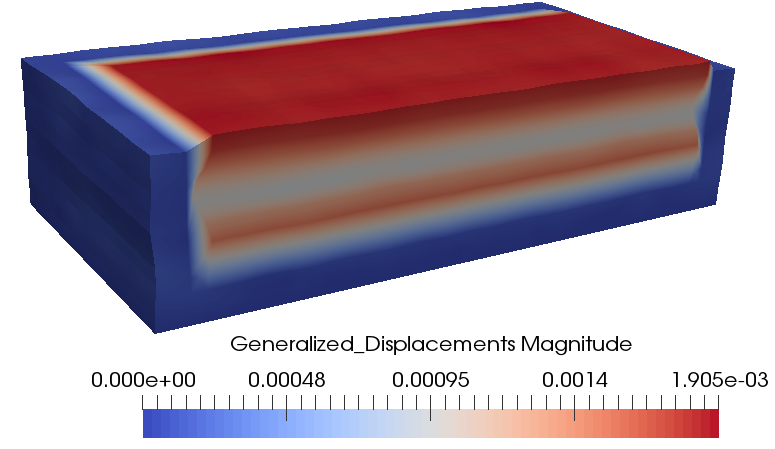
\includegraphics[width = 10cm]{./Figure-files/Day2/Deconvolution_3by1D_Motions/Free_fields_3D_model_with_DRM/motion3D_DRM3D_free_field.png}
  \caption{Simulation Model}
  \label{fig_decon_3D_motion_3D_model_results_free_field}
\end{figure}


% ******************************************************************
% ******************************************************************
% ******************************************************************
\clearpage
\newpage
\subsection{Free field 3D model, deconvolution  3$\times$1D motion, solid model with DRM}
\label{Earthquake_Soil-structure_interaction_3D_model_with_DRM3}

The Real-ESSI input files for this example are available 
\href{https://github.com/yuan-energy/Real-ESSI-Short-Course-Examples/tree/master/short-course-examples/Day2/Deconvolution_3by1D_Motions/Earthquake_Soil-structure_interaction_3D_model_with_DRM}{HERE}. 
The compressed package of Real-ESSI input files for this example is available 
\href{https://github.com/yuan-energy/Real-ESSI-Short-Course-Examples/blob/master/short-course-examples/Day2/Deconvolution_3by1D_Motions/Earthquake_Soil-structure_interaction_3D_model_with_DRM/Earthquake_Soil-structure_interaction_3D_model_with_DRM.tgz?raw=true}{HERE}. 

The Modeling parameters are listed.
\begin{itemize}
  \item Elastic Soil Material Properties 
  \begin{itemize}
    \item Mass density, $\rho$, \enspace \enspace 2000 $kg/m^3$
    \item Young's modulus, $E$, \enspace \enspace 200 MPa
    \item Poisson's ratio, $\nu$, \enspace \enspace 0.1
  \end{itemize}
  \item Elastic Structure Material Properties 
  \begin{itemize}
    \item Mass density, $\rho$, \enspace \enspace 2500 $kg/m^3$
    \item Young's modulus, $E$, \enspace \enspace 20 GPa
    \item Poisson's ratio, $\nu$, \enspace \enspace 0.1
  \end{itemize}
\end{itemize}

\begin{figure}[H]
  \centering
  \includegraphics[width = 8cm]{./Figure-files/Day2/Deconvolution_3by1D_Motions/Earthquake_Soil-Structure_Interaction_3D_Model_with_DRM/overview.png}
  \caption{Simulation Model}
  \label{fig_decon_1D_motion_3D_model3}
\end{figure}


The illustration results of the simulation is shown in Fig.~\ref{fig_decon_3D_motion_3D_model_results_structure}.
As shown in the results, outside the DRM layer, there is no outgoing waves. 

\begin{figure}[H]
  \centering
  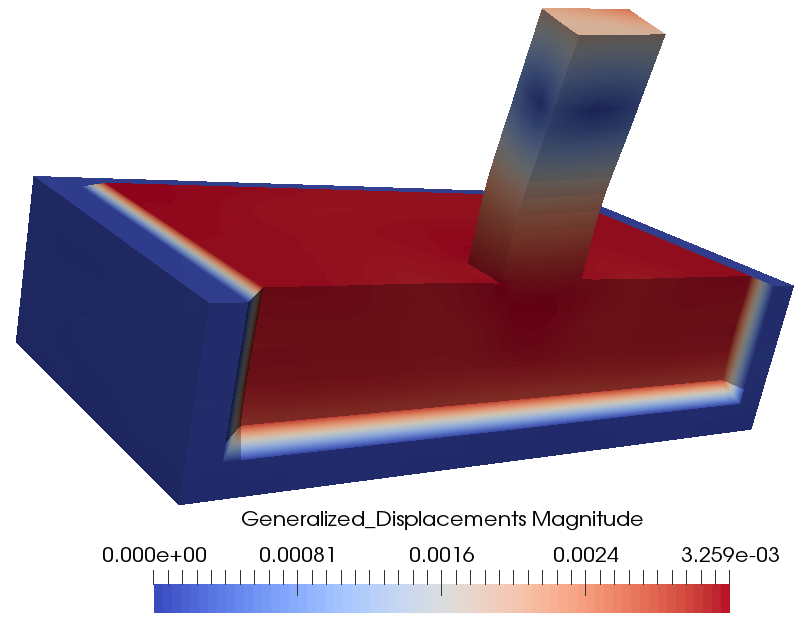
\includegraphics[width = 10cm]{./Figure-files/Day2/Deconvolution_3by1D_Motions/Earthquake_Soil-Structure_Interaction_3D_Model_with_DRM/DRM3D_motion3D_structure.png}
  \caption{Simulation Model}
  \label{fig_decon_3D_motion_3D_model_results_structure}
\end{figure}





% ******************************************************************
% ******************************************************************
% ******************************************************************
\clearpage
\newpage
\subsection{ESSI 3D building model, deconvolution  3$\times$1D motion, shell model with DRM}
\label{Earthquake_Soil-Structure_Interaction_3D_Model_with_DRM4}

The Real-ESSI input files for this example are available 
\href{https://github.com/yuan-energy/Real-ESSI-Short-Course-Examples/tree/master/short-course-examples/Day2/Deconvolution_3by1D_Motions/Shell_Structure_Soil_Interaction_3D_DRM}{HERE}. 
The compressed package of Real-ESSI input files for this example is available 
\href{https://github.com/yuan-energy/Real-ESSI-Short-Course-Examples/blob/master/short-course-examples/Day2/Deconvolution_3by1D_Motions/Shell_Structure_Soil_Interaction_3D_DRM/Shell_Structure_Soil_Interaction_3D_DRM.tgz?raw=true}{HERE}. 

The Modeling parameters are listed.
\begin{itemize}
  \item Elastic Soil Material Properties 
  \begin{itemize}
    \item Mass density, $\rho$, \enspace \enspace 2000 $kg/m^3$
    \item Young's modulus, $E$, \enspace \enspace 200 MPa
    \item Poisson's ratio, $\nu$, \enspace \enspace 0.1
  \end{itemize}
  \item Elastic Structure Material Properties 
  \begin{itemize}
    \item Mass density, $\rho$, \enspace \enspace 2500 $kg/m^3$
    \item Young's modulus, $E$, \enspace \enspace 20 GPa
    \item Poisson's ratio, $\nu$, \enspace \enspace 0.1
  \end{itemize}
\end{itemize}

\begin{figure}[H]
  \centering
  \includegraphics[width = 8cm]{./Figure-files/Day2/Deconvolution_3by1D_Motions/Shell_Structure_Soil_Interaction_3D_DRM/overview.png}
  \caption{Simulation Model}
  \label{fig_decon_3by1D_motion_3D_model_shell}
\end{figure}


The illustration results of DRM 3D shell Structure Model under 1D motion is shown 
in Fig.~\ref{fig_decon_3by1D_motion_3D_model_solid_shell_structure}. 

\begin{figure}[H]
  \centering
  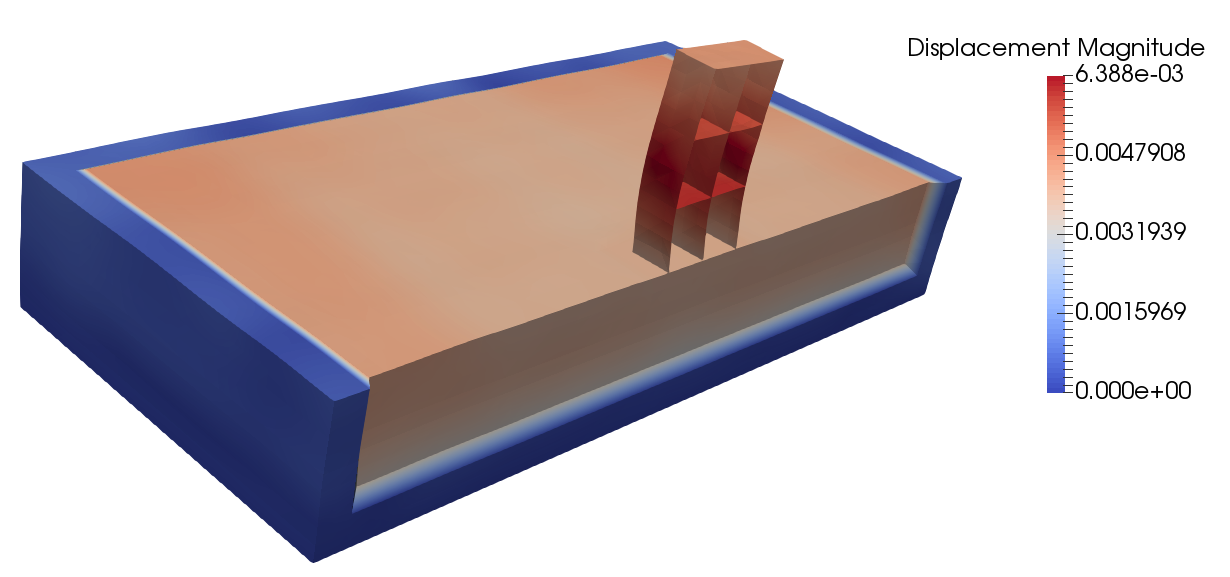
\includegraphics[width = 10cm]{./Figure-files/Day2/Deconvolution_3by1D_Motions/Shell_Structure_Soil_Interaction_3D_DRM/DRM3D_motion3D_shell.png}
  \caption{Simulation Model}
  \label{fig_decon_3by1D_motion_3D_model_solid_shell_structure}
\end{figure}


















% ******************************************************************
% ******************************************************************
% ******************************************************************
\clearpage
\newpage
\section{Mesh Dependence of Wave Propagation Frequencies}
\label{Convolution_Motions}


The Real-ESSI input files for this example are available 
\href{https://github.com/yuan-energy/Real-ESSI-Short-Course-Examples/tree/master/short-course-examples/Day2/Convolution_Motions}{HERE}. 
The compressed package of Real-ESSI input files for this example is available 
\href{https://github.com/yuan-energy/Real-ESSI-Short-Course-Examples/blob/master/short-course-examples/Day2/Convolution_Motions/Convolution_Motions.tgz?raw=true}{HERE}. 


Show the mesh dependence of high frequency wave with Ormsby wavelet.

\begin{figure}[H]
  \centering
  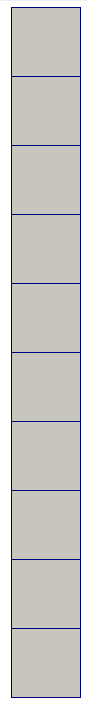
\includegraphics[width = 0.5cm]{./Figure-files/Day2/Convolution_Motions/overview.png}
  \caption{Simulation Model}
  \label{fig_decon_1D_motion_3D_model4}
\end{figure}

The illustration results of mesh dependence is shown in Fig.~\ref{fig_day2_convolution_time_freq}.

\begin{figure}[H]
  \centering
  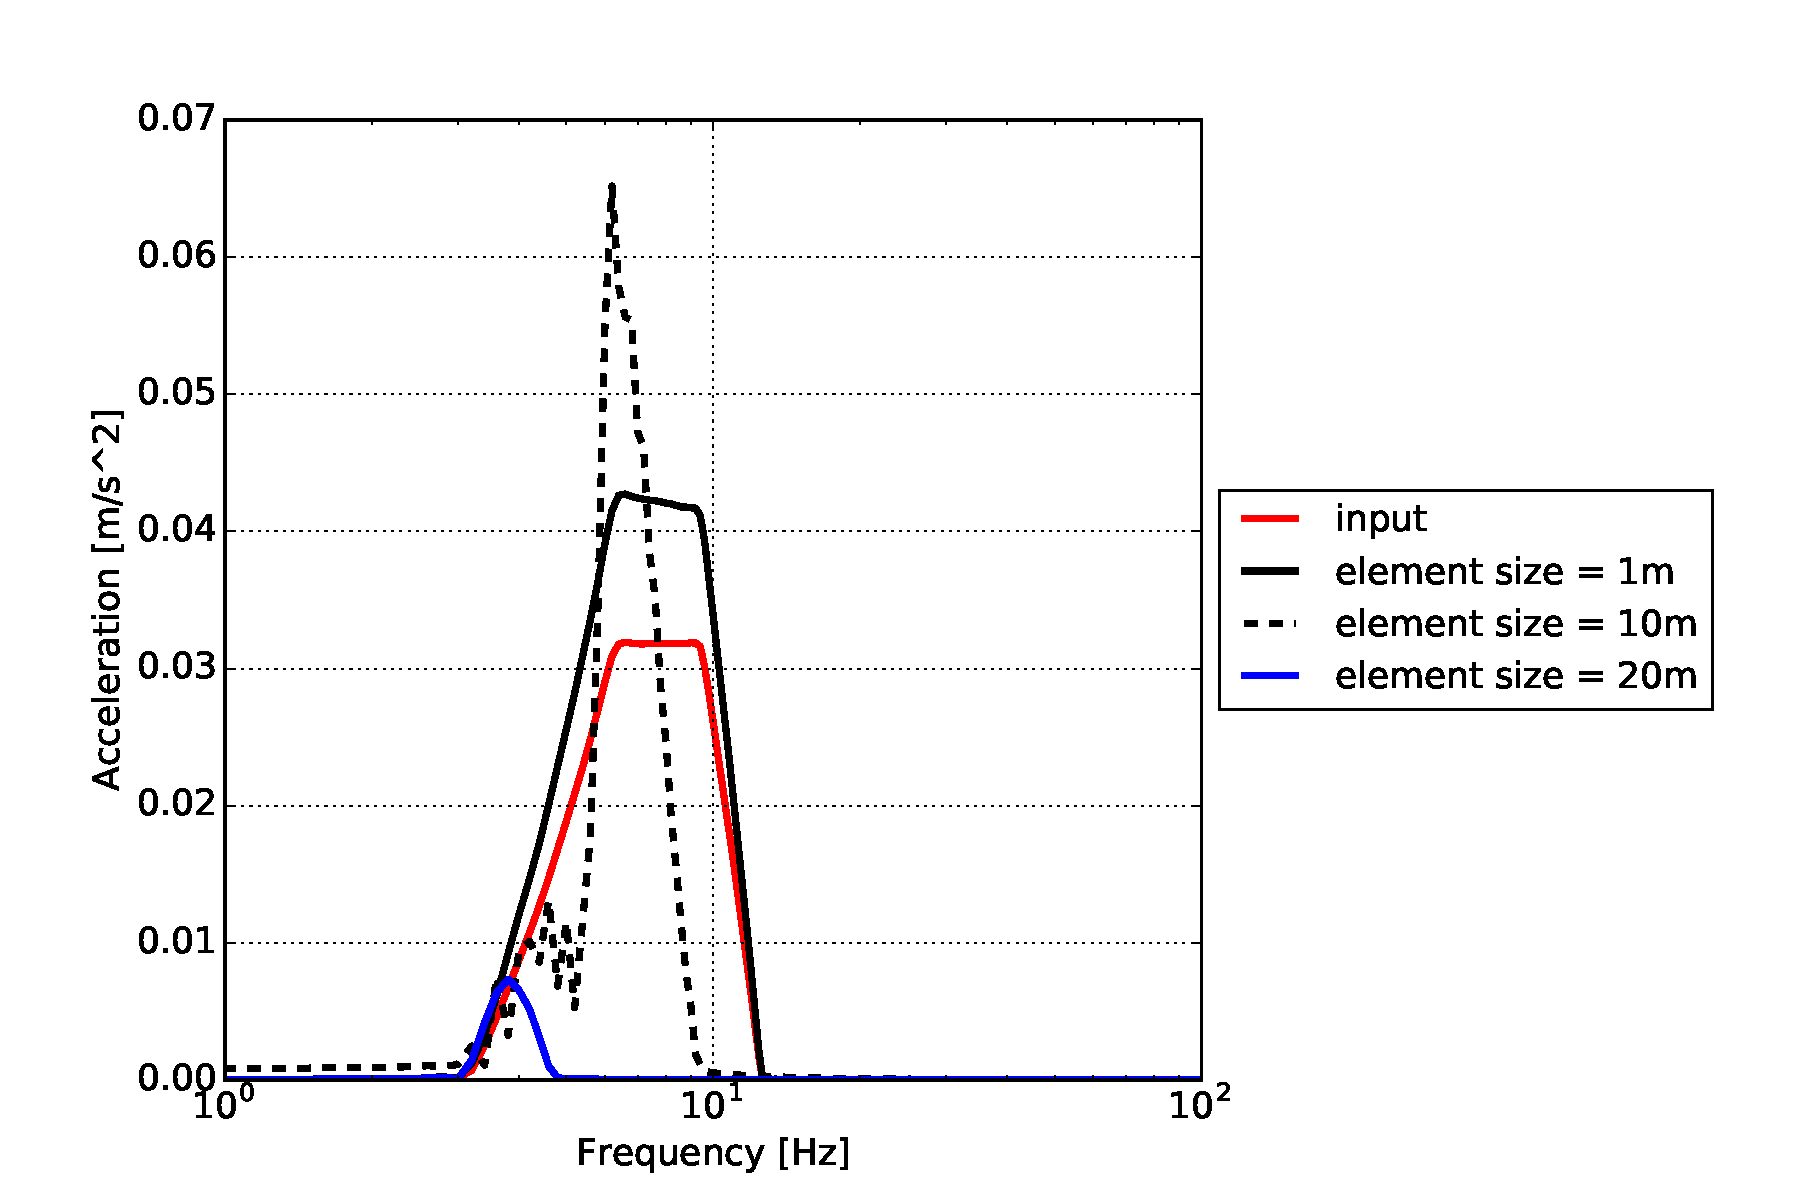
\includegraphics[width = 12cm]{./Figure-files/Day2/Convolution_Motions/top_acc_feq_all.pdf}
  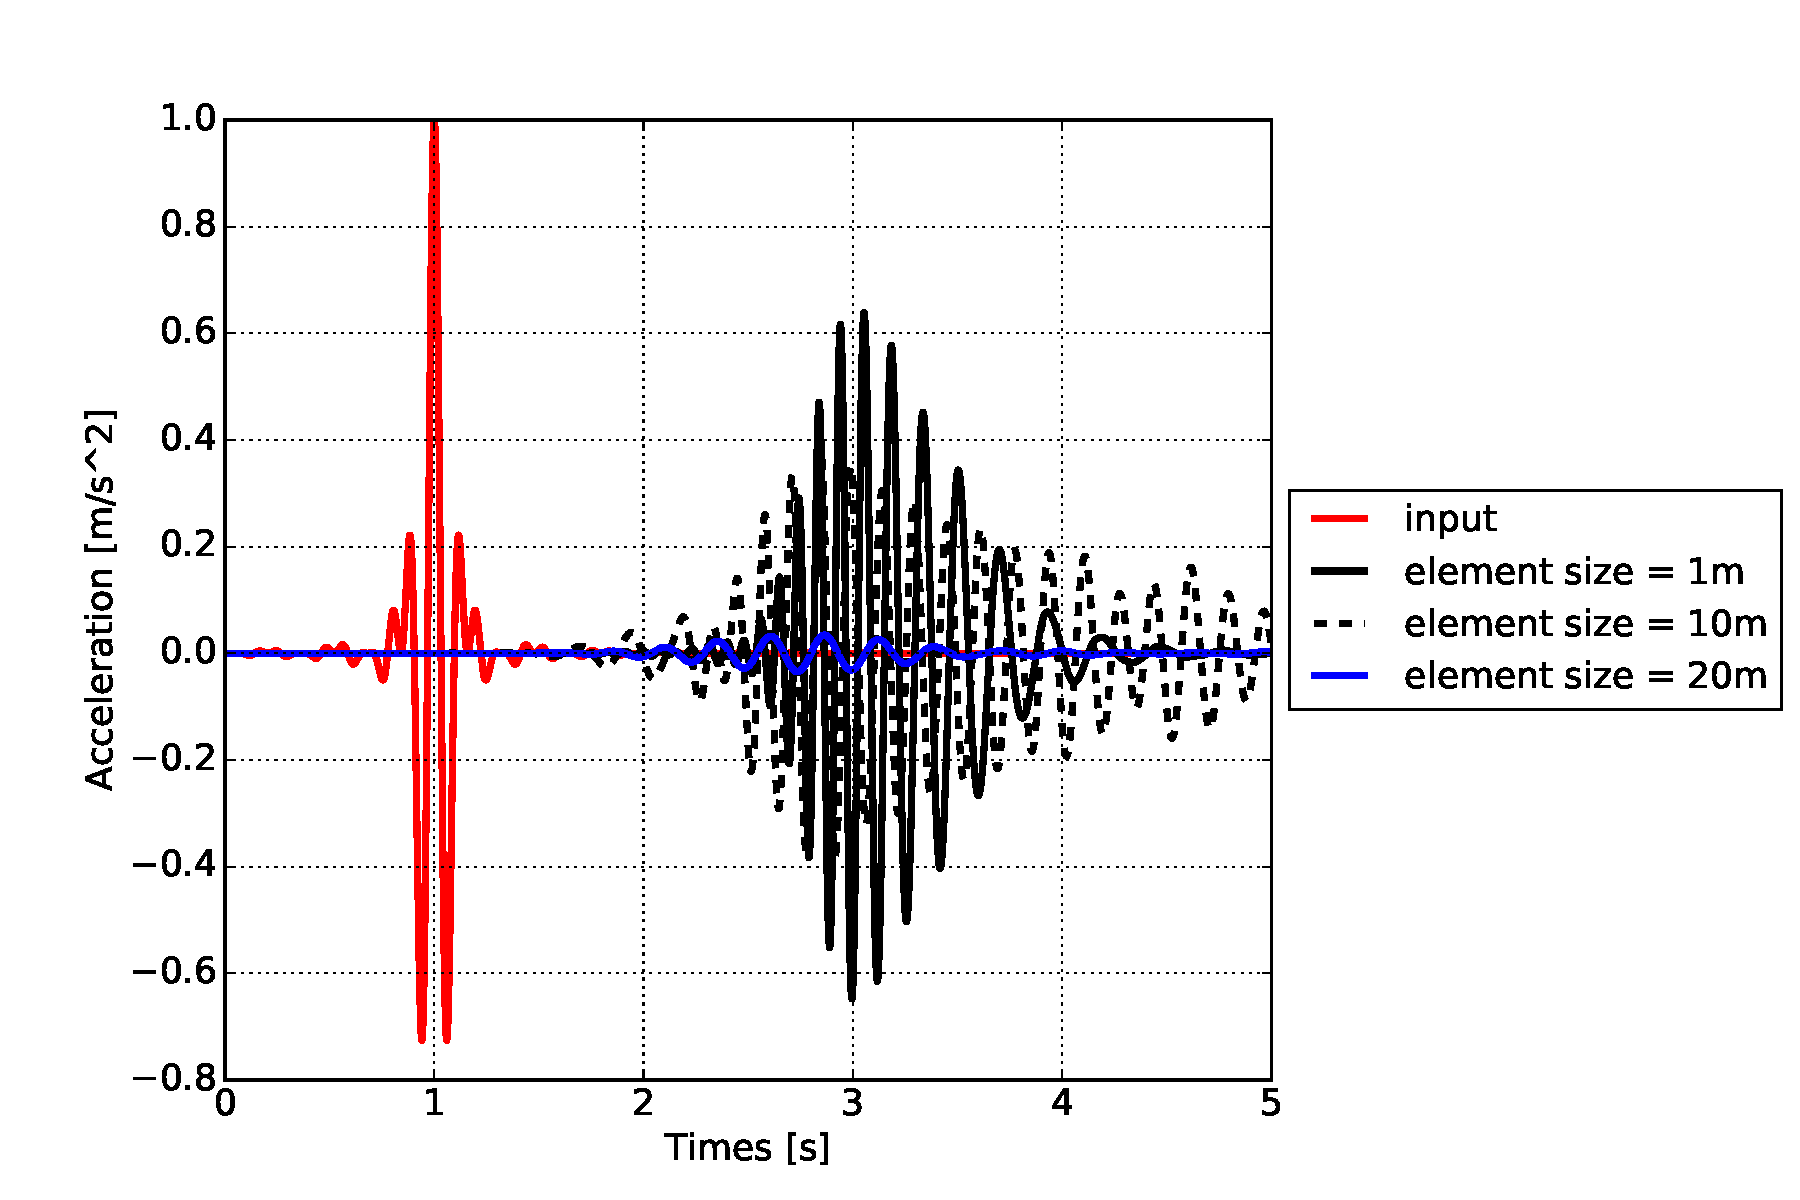
\includegraphics[width = 12cm]{./Figure-files/Day2/Convolution_Motions/top_acc_time_all.pdf}
  \caption{Convolution Results and Mesh Dependence}
  \label{fig_day2_convolution_time_freq}
\end{figure}

































% ******************************************************************
% ******************************************************************
% ******************************************************************
\clearpage
\newpage
\section{Apply 3D Motions from SW4}
\label{Apply_3D_Motions_from_SW4}

\subsection{Free field 3D model, 3D motion, model with DRM}
\label{Free_fields_3D_model_with_DRM3}


The Real-ESSI input files for this example are available 
\href{https://github.com/yuan-energy/Real-ESSI-Short-Course-Examples/tree/master/short-course-examples/Day2/Apply_3D_Motions_from_SW4/Free_fields_3D_model_with_DRM}{HERE}. 
The compressed package of Real-ESSI input files for this example is available 
\href{https://github.com/yuan-energy/Real-ESSI-Short-Course-Examples/blob/master/short-course-examples/Day2/Apply_3D_Motions_from_SW4/Free_fields_3D_model_with_DRM/Free_fields_3D_model_with_DRM.tgz?raw=true}{HERE}. 


\begin{figure}[H]
  \centering
  \includegraphics[width = 8cm]{./Figure-files/Day2/Apply_3D_Motions_from_SW4/Free_fields_3D_model_with_DRM/overview.png}
  \caption{Simulation Model}
  \label{fig_decon_1D_motion_3D_model5}
\end{figure}


% The illustration results of free field DRM 3D Model under 1D motion is shown 
% in Fig.~\ref{fig_day2_DRM3D_results}. 

% \begin{figure}[H]
%   \centering
%   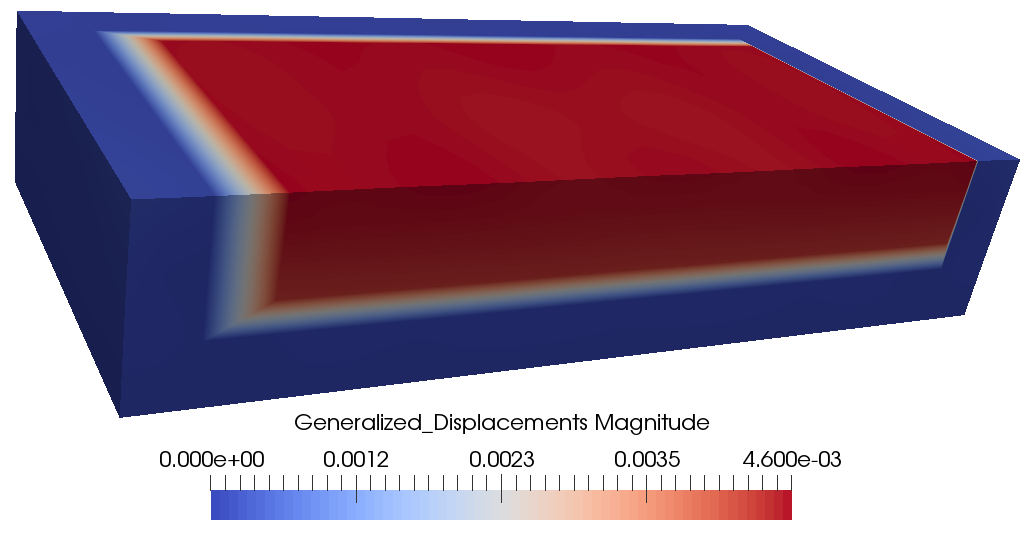
\includegraphics[width = 10cm]{./Figure-files/Day1/Preprocess_examples_with_Gmsh/example4/DRM3D_results.png}
%   \caption{Simulation Model DRM 2D}
%   \label{fig_day2_DRM3D_results}
% \end{figure}



% ******************************************************************
% ******************************************************************
% ******************************************************************
\clearpage
\newpage
\subsection{ESSI 3D building model, 3D motion, solid model with DRM}
\label{Earthquake_Soil-Structure_Interaction_3D_Model_with_DRM5}

The Real-ESSI input files for this example are available 
\href{https://github.com/yuan-energy/Real-ESSI-Short-Course-Examples/tree/master/short-course-examples/Day2/Apply_3D_Motions_from_SW4/Earthquake_Soil-Structure_Interaction_3D_Model_with_DRM}{HERE}. 
The compressed package of Real-ESSI input files for this example is available 
\href{https://github.com/yuan-energy/Real-ESSI-Short-Course-Examples/blob/master/short-course-examples/Day2/Apply_3D_Motions_from_SW4/Earthquake_Soil-Structure_Interaction_3D_Model_with_DRM/Earthquake_Soil-Structure_Interaction_3D_Model_with_DRM.tgz?raw=true}{HERE}. 


\begin{figure}[H]
  \centering
  \includegraphics[width = 8cm]{./Figure-files/Day2/Apply_3D_Motions_from_SW4/Earthquake_Soil-Structure_Interaction_3D_Model_with_DRM/overview.png}
  \caption{Simulation Model}
  \label{fig_decon_1D_motion_3D_model6}
\end{figure}


% The illustration results of DRM 3D Solid Structure Model  under 1D motion is shown 
% in Fig.~\ref{fig_decon_1D_motion_3D_model_solid_structure}. 

% \begin{figure}[H]
%   \centering
%   \includegraphics[width = 10cm]{./Figure-files/Day2/Apply_3D_Motions_from_SW4/Earthquake_Soil-Structure_Interaction_3D_Model_with_DRM/DRM3D_results_1Dmotion.png}
%   \caption{Simulation Model}
%   \label{fig_decon_1D_motion_3D_model_solid_structure}
% \end{figure}




% ******************************************************************
% ******************************************************************
% ******************************************************************
\clearpage
\newpage
\subsection{ESSI 3D building model, 3D motion, shell model with DRM}
\label{Earthquake_Soil-Structure_Interaction_3D_Model_with_DRM6}

The Real-ESSI input files for this example are available 
\href{https://github.com/yuan-energy/Real-ESSI-Short-Course-Examples/tree/master/short-course-examples/Day2/Apply_3D_Motions_from_SW4/Shell_Structure_Soil_Interaction_3D_DRM}{HERE}. 
The compressed package of Real-ESSI input files for this example is available 
\href{https://github.com/yuan-energy/Real-ESSI-Short-Course-Examples/blob/master/short-course-examples/Day2/Apply_3D_Motions_from_SW4/Shell_Structure_Soil_Interaction_3D_DRM/Shell_Structure_Soil_Interaction_3D_DRM.tgz?raw=true}{HERE}. 


\begin{figure}[H]
  \centering
  \includegraphics[width = 8cm]{./Figure-files/Day2/Apply_3D_Motions_from_SW4/Shell_Structure_Soil_Interaction_3D_DRM/overview.png}
  \caption{Simulation Model}
  \label{fig_decon_1D_motion_3D_model_shell2}
\end{figure}


% The illustration results of DRM 3D shell Structure Model under 1D motion is shown 
% in Fig.~\ref{fig_decon_1D_motion_3D_model_solid_shell_structure}. 

% \begin{figure}[H]
%   \centering
%   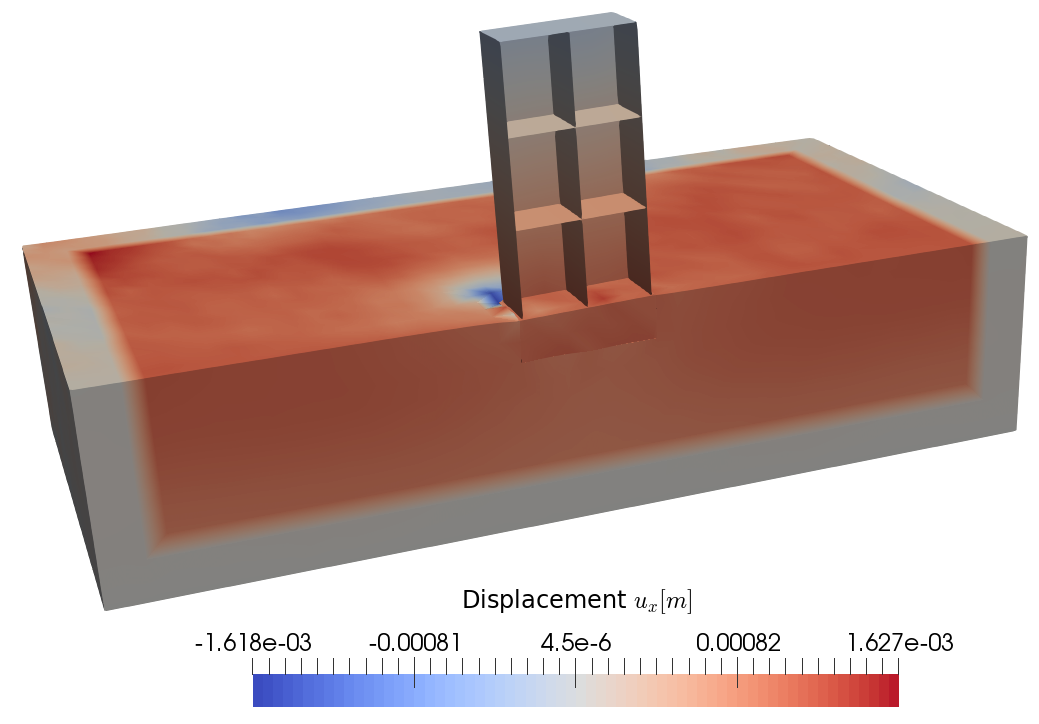
\includegraphics[width = 10cm]{./Figure-files/Day2/Apply_3D_Motions_from_SW4/Shell_Structure_Soil_Interaction_3D_DRM/shell_DRM3D.png}
%   \caption{Simulation Model}
%   \label{fig_decon_1D_motion_3D_model_solid_shell_structure}
% \end{figure}

